\chapter{Digital signal processing component} \label{chap:hdl}

This chapter is dedicated to the presentation of the developed digital signal processing module, which consists on an effort to improve a system created in a previous project.

In the first part, the developed hardware module is introduced which receives acoustic signals from the hydrophones and computes the phase differences between them. The design decisions are explained along with some mathematical notions and block diagrams that represent the projected system. 

Then, two particular phenomena inherent to the system are addressed, regarding a phase ambiguity issue and the influence of the Doppler effect. These are defined and conclusions are given based on the presented rationale.

\section{HDL Module Architecture} \label{subchap:HDL module}

The USBL system was developed in previous dissertations and research work, which can be better understood in \cite{afonso-thesis}. Briefly, the system consists on a transducer of four hydrophones forming a 3D array deployed on the mule AUV. This array will receive the same signal wave front. The system then calculates the cross-correlation between the received and expected signals, which is a BPSK modulated binary sequence. The cross-correlation peak indicates the distance between AUVs and it is calculated with timing resolution corresponding to 1 sampling period of the acquired signal, which in the developed systems corresponds approximately to 6mm (with a sampling frequency of 244kHz).

Since we are referring to an USBL system and due to the limitations in dimension of the AUV that will integrate this system, the hydrophones have to be placed within a few centimeters from each other. For this reason, the obtained time resolution by using only the cross-correlation, corresponding to a maximum distance accuracy of approximately 6mm, will not be enough for the calculation of the angle of arrival of the sound wave. Thus, in this thesis it is intended to refine this measurement by additionally calculating the phase differences of the arriving signals to each hydrophone. Upon having this measurement refined, the phase differences, as well as additional data from modules already implemented, will serve as input in a software mechanism that estimates the angle of arrival of the received signal to the hydrophone array.

The proposed module receives 4 inputs, which correspond to the received signals in each hydrophone, and outputs the average phase difference between all combinations of hydrophone pairs. This model was developed using Verilog, which is a commonly used hardware description language, and all designed components were validated with testbenches through simulations.

The module is a synchronous system, since all elements are synchronized by a global clock. It follows a sequential logic, so it is time dependent and contains memory elements. All sub components receive an input from a memory element triggered by the clock and originates an output which is also saved in a memory element triggered by the clock, in order to avoid capturing unstable signals.

\subsection{Module components}

The overall system is composed by four main functional blocks, represented in \ref{fig:module-all}. The hydrophone array, composed by hydrophones $i$ with $i=\{1,2,3,4\}$, receives the signals in each sensor and sends them to an Analog to Digital Converter (ADC). The generated digital signals are then input of a module based on a Hilbert transform, which converts the real signal to a complex representation. These are then multiplexed so each pair of real, $Re_i$, and imaginary, $Im_i$, components are input in a CORDIC \cite{cordic-def} block, responsible for computing the signal's phase, $phase_i$. Afterwards, it is possible to calculate the phase differences for all combinations of pairs, $diff_{ij}$ with $i \neq j$, which are finally averaged in order to obtain a more stable phase difference, $\Delta phase_{ij}$.

The module receives a global clock and reset which are connected to all registers, as well as an enable signal which allows the sub modules to capture new inputs and release the outputs synchronically.

\begin{figure}[!htbp]
	\makebox[\textwidth][c]{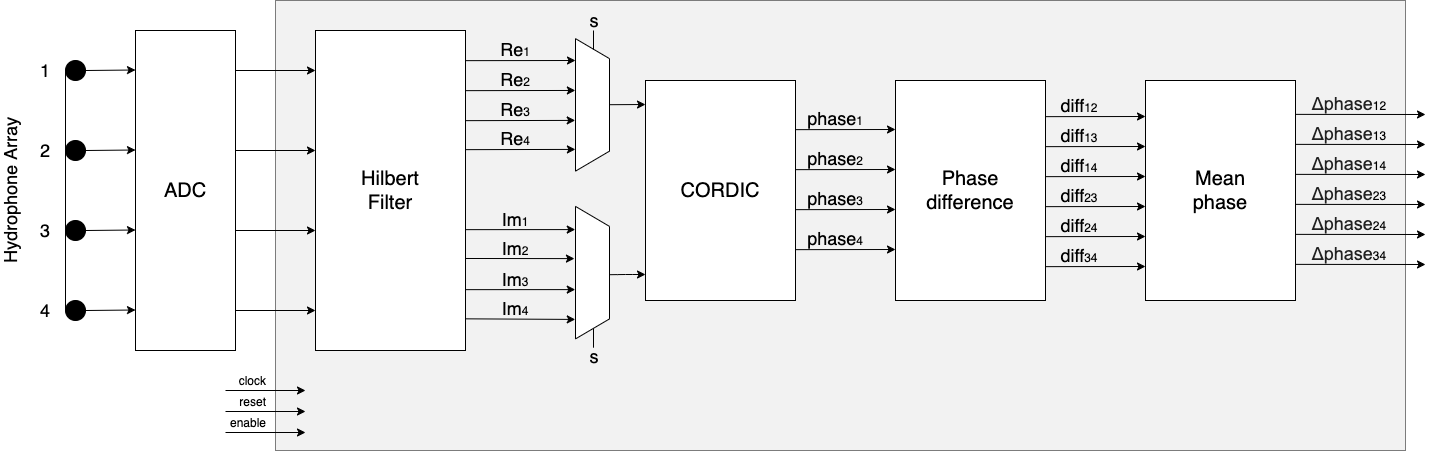
\includegraphics[width=1\textwidth]{figures/hdl-diagram-all}}
	\captionsetup{justification=centering,margin=2cm}
	\caption{Top level architecture}
	\label{fig:module-all}
\end{figure}

Considering that the ADC receives signals at a frequency of $244 kHz$ and outputs at a frequency of $125MHz$, then the system received a new input every 512 clock cycles. Assuming that a latency of a few inputs is tolerable, then each sub component can use up to 512 clock cycles since receiving an input until generating an output. As the performed calculations are fairly simple, the available clock cycles are more than enough to originate the outputs, therefore this architecture does not involve time constraints. Instead, it focuses on minimizing the used area since it is part of a complex system that already uses a substantial part of the FPGA resources.

In order to describe the efforts to minimize the used area, all module sub components are detailed next, namely the Hilbert filter, CORDIC, Phase difference and Mean phase.

\subsubsection{Hilbert Filter}

The signals coming from the ADC are purely real so they need to be converted to their analytic representation. This is achieved by using a module based on a Hilbert FIR filter, which derives the complex representation by comprehending the original real signal and its Hilbert transform. 

The Hilbert transform definition is given by (\ref{eq:hilbert_integral}) \cite{hilbert-def}, where $x(t)$ is the original signal and $P$ is the Cauchy principal value.

\begin{eqnarray}
	H(x)(t) = \frac{1}{\pi} \ P \int_{-\infty}^{\infty}\frac{x(\tau)}{t-\tau}d\tau
	\label{eq:hilbert_integral}
\end{eqnarray}

The notation for a digital N-th order FIR filter can be expressed by equation 1 in \cite{hilbert-fpga}. Assuming a eighth-order filter that can be approximated with alternated zero coefficients, then equation (\ref{eq:hilbert_imeq}) represents the imaginary part of the signal, $Imag_0$, for a sample $x_{0}$ received in the present moment , assuming $x_{-i}$ as the input samples received $i$ sampling periods before. Then, (\ref{eq:hilbert_reeq}) represents the real part of the signal for the same sample, which simply consists on delaying four sampling periods the original signal.

\begin{eqnarray}
	&Imag_0 = a_{1} \ x_{-1} +a_{3} \ x_{-3} + a_{5} \ x_{-5} + a_{7} \ x_{-7} \\
	\label{eq:hilbert_imeq}
	&Real_0 = x_{-4} 
	\label{eq:hilbert_reeq}
\end{eqnarray}

The eighth-order coefficients can be obtained through a design tool, such as the \textit{designfilt} function on MATLAB, and respect an odd anti-symmetry, i.e. $a_{1} = - a_{7}$ and $a_{3} = - a_{5}$.

In order to implement this filter, the most common approach is to use a chain of registers that integrate multiple adders and multipliers, so that the calculations take less clock cycles to obtain a valid result, similarly to the work in \cite{hilbert-fpga}. However, since the goal of this implementation is to minimize area, then an alternative approach was formulated which uses only one multiplier and one adder. As can be observed in the filter equation, all odd samples need to be multiplied by a coefficient and summed with each other. Therefore, by using a circular shifting register chain \ref{fig:hilbert-chai} for each arriving signal, it is possible to position each of the buffer chain's samples in register $x_8$, which is used for external calculations.

\begin{figure}[!htbp]
	\makebox[\textwidth][c]{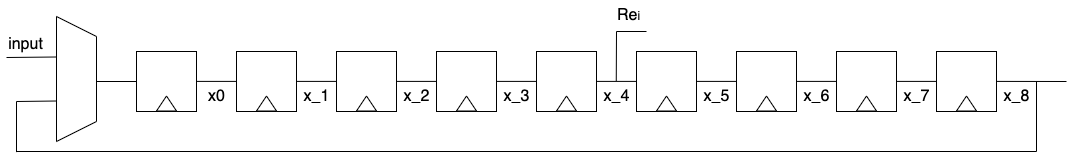
\includegraphics[width=0.9\textwidth]{figures/hilbert-filt-chain}}
	\captionsetup{justification=centering,margin=2cm}
	\caption{Hilbert Filter circular shifting register chain}
	\label{fig:hilbert-chai}
\end{figure}

In a more comprehensive view, the register chains $HF_{Ci}$ are integrated with the remaining block elements as represented in \ref{fig:hilbert-all}. The module receives four signals as input and outputs the real and imaginary components, $Real_i$ and $Imag_i$, for each of them.

\begin{figure}[!htbp]
	\makebox[\textwidth][c]{\includegraphics[width=0.9\textwidth]{figures/hilbert-filt-all}}
	\captionsetup{justification=centering,margin=2cm}
	\caption{Hilbert Filter block diagram}
	\label{fig:hilbert-all}
\end{figure}

The implementation contains a series of design decisions that lead to decreased area occupation, presented as follows :

\begin{itemize}
	\item The four register chains are multiplexed so that the module needs only one multiplier and one adder to calculate the Hilbert transform for all signals;
	
	\item Since the coefficients have odd symmetric pairs, then only two variables and their symmetric value are needed, which will be referred as $c_a$, $c_b$, -$c_a$ and -$c_b$. For even samples, associated with coefficients equal to zero, a controller unit is responsible for skipping the multiplication, which saves energy. For odd samples, the control unit alternates between the positive and negative coefficients to be multiplied. The control unit settings are summarized in table \ref{tab:coeffs-control-unit} for each register chain sample. 
	
	\begin{table}[!htbp] %use H to adjust
		\begin{center}
			\makebox[\textwidth]{
				\begin{tabular}{ c | c  c  }
					%\hline
					\toprule
					\multicolumn{1}{c|}{} & Multiplier Coefficient  & Adder mode\\	
					\midrule
					\multicolumn{1}{c|}{$a_0$} &  0 & -\\
					\midrule
					\multicolumn{1}{c|}{$a_1$} &  -$c_a$ & -\\
					\midrule
					\multicolumn{1}{c|}{$a_2$} &  0 & -\\
					\midrule
					\multicolumn{1}{c|}{$a_3$} &  -$c_b$ & -\\
					\midrule
					\multicolumn{1}{c|}{$a_4$} & 0 & +\\
					\midrule
					\multicolumn{1}{c|}{$a_5$} &  $c_b$ & +\\
					\midrule
					\multicolumn{1}{c|}{$a_6$} & 0 &+ \\
					\midrule
					\multicolumn{1}{c|}{$a_7$} &  $c_a$ & +\\
					\midrule
					\multicolumn{1}{c|}{$a_8$} & 0 &+ \\
					\bottomrule 
			\end{tabular}}
			\caption{Hilbert filter control unit settings for each processed sample}
			\label{tab:coeffs-control-unit}
		\end{center}
	\end{table}
	
	\item The negative coefficients are achieved by subtracting the result of $a_{i} \ x_{-i}$, i.e. negating the adder, so only one adder block is necessary;
	
	\item A register is placed after the adder so that it interactively accumulates the value that is correspondent to the imaginary component $Im_i$ after the full chain circle shifting.
	
\end{itemize}

Having cleared the implementation details, it is possible to deduce that each $HF_{Ci}$ takes 9 clock cycles to be processed. Therefore, the entire calculation takes $9 \times 4$ clock cycles plus one additional cycle to update the outputs.

An additional detail can be pointed out regarding the impulse response of the Hilbert filter. For high filter orders, the impulse response does not suffer substantial attenuation. However, for an eighth-order filter there is a visible gain attenuation and overflow, which leads to wrong results if the dynamic range is not adequate. Therefore, it is possible to create a mechanism that applies variable gain to the filter output depending on the frequency so that it is possible to make it constant and avoid this issue.

\subsubsection{CORDIC}

The CORDIC algorithm is used for real-time trigonometric and exponential calculations, as well as polar to rectangular conversions and vice-versa, using iterative vector rotations. 

The implemented CORDIC module has a sequential structure, as it occupies the least area, and it is responsible for receiving the real and imaginary components of a signal and outputting its phase. There are two possible modes of operation from which it is used the vectoring mode (VM), whose algorithm computes the magnitude and phase of the input vector ($(x_0, y_0)$) from the x-axis \cite{cordic-def}. This is achieved by iteratively approximating the phase through angle microrotations of $\alpha_i = \pm atan(2^{-i})$ which are summed originating an approximated phase. The result is given in a 16 bit value, which is composed by 9 bits for the integer part and 7 bits that represent the fractional portion. 

The CORDIC iterations are expressed by (\ref{eq:cordic-iter-x}), (\ref{eq:cordic-iter-y}) and (\ref{eq:cordic-iter-z}) for $d_i$ belonging to \{-1,1\}.

\begin{eqnarray}
	& x_{i+1} = x_i - d_i \ 2^{-1} \ y_i
	\label{eq:cordic-iter-x}  \\
	& y_{i+1} = y_i + d_i \ 2^{-1} \ x_i
	\label{eq:cordic-iter-y} \\
	& z_{i+1} = z_i - d_i \ \alpha_i
	\label{eq:cordic-iter-z}
\end{eqnarray}

The CORDIC logic uses a 16 element ROM (Read-Only Memory) that stores the $atan(2^{-1})$ values required for the algorithm. Additionally, another sub component provides a binary counter that defines the number of performed iterations and it is also responsible for generating the address to access the ROM. 

Considering that the CORDIC module uses 16 clock cycles to run through the entire ROM and one additional cycle to update the outputs, there are still many remaining clock cycles from the 512 available. Therefore, the design uses only one CORDIC module with multiplexed inputs so the process takes $17 \times 4$ plus one, to update the global outputs, in a total of 69 clock cycles.

\subsubsection{Phase difference}

This sub module is responsible for computing the phase differences between the previously determined signals' phases, $phase_i$. For four inputs $phase_i$, it is generated the difference between all combinations of hydrophones, resulting in six pairs: 12, 13, 14, 23, 24 and 34.

This is achieved using a single subtractor which has multiplexed inputs so that the calculations can be executed within the 512 clock cycles with only one block of hardware, instead of dedicated subtractor for each calculation. 

The result is given in a 16 bit value, which is composed by 10 bits for the integer part and 6 bits that represent the fractional portion. 

\subsubsection{Mean phase}

Finally, the last sub module is responsible for accumulating N samples of the phase difference $diff_{ij}$ and calculate a mean phase difference, so that the value is less affected by variations.  Parameter N depends on a customizable input $k$ where $2^k = N$. 

The averaged phase differences is given in a 16 bit value, which is composed by 10 bits for the integer part and 6 bits that represent the fractional portion. 

\subsection{Performance and resource analysis}

The module that computed the phase differences is intended to decrease the used area, thus the used components, in order to improve an existing version of a design with the same purpose. The previous version used approximately 10k slice registers and 6k slice LUTs, whereas the present architecture reduced these numbers to 1216 and 1432, respectively, consisting of a successful improvement.

This module was integrated in the global complex system which was subjected to field tests in the water. Although the ground truth was not rigorous, after processing the results, it was roughly estimated that the phase differences do not vary more than $15^{\circ}$, which corresponds to approximately $2.5mm$. Comparatively to the previous $6mm$ of time resolution achieved through correlation, this result constitutes an improvement. Therefore, after this initial analysis, it is considered that the process which uses the phase differences along with the correlation is expected to improve the angle of arrival estimation precision.

%-------------------------------------------------------------------------------------
%-------------------------------------------------------------------------------------
\section{Inherent phenomena}

Systems that are implemented in a controlled environment may deal with issues that arise when integrated in real applications. Therefore, in this section two concepts are explored: phase ambiguity and the Doppler effect .

\subsection{Phase Ambiguity}

To improve the determination of the time difference of arrival between the hydrophones, the implemented signal processing system calculates the difference of phase between the received signals. As the distance between hydrophones is always larger than the wavelength of the acoustic signals used, the phase alone is not sufficient to determine the time difference of arrival. Time-domain correlation is thus combined with the phase difference calculation to remove the ambiguity and obtain a time difference of arrival with a time resolution that is far beyond the sampling period used in the digital signal processing system.

When the information about the time of arrival of a signal is available, it is relatively easy to estimate the distance between the transmitter and the receiver since there can be a direct conversion between them. However, when dealing with phase differences, there is no exact time notion, so it is necessary to start by defining a reference point. 

Considering sinusoidal signals, when we have an array with four hydrophones spatially placed to form a 3D layout, the signal that is arriving to each  hydrophone in different times consequently have different phases. However, since sinusoidal signals are periodic, this means that for different signal periods the same phase value is observed, i.e. the phase is ambiguous \ref{fig:phasediff}. In this illustration, $\alpha$ represents the observable phase difference of hydrophone $H_4$ to the reference point $H_1$. However, the actual time difference which is intended to obtain, $\Delta t_4$, is one period of the signal, $\lambda$, added to the observable phase $\alpha$.

\begin{figure}[!htbp]
	\centering
	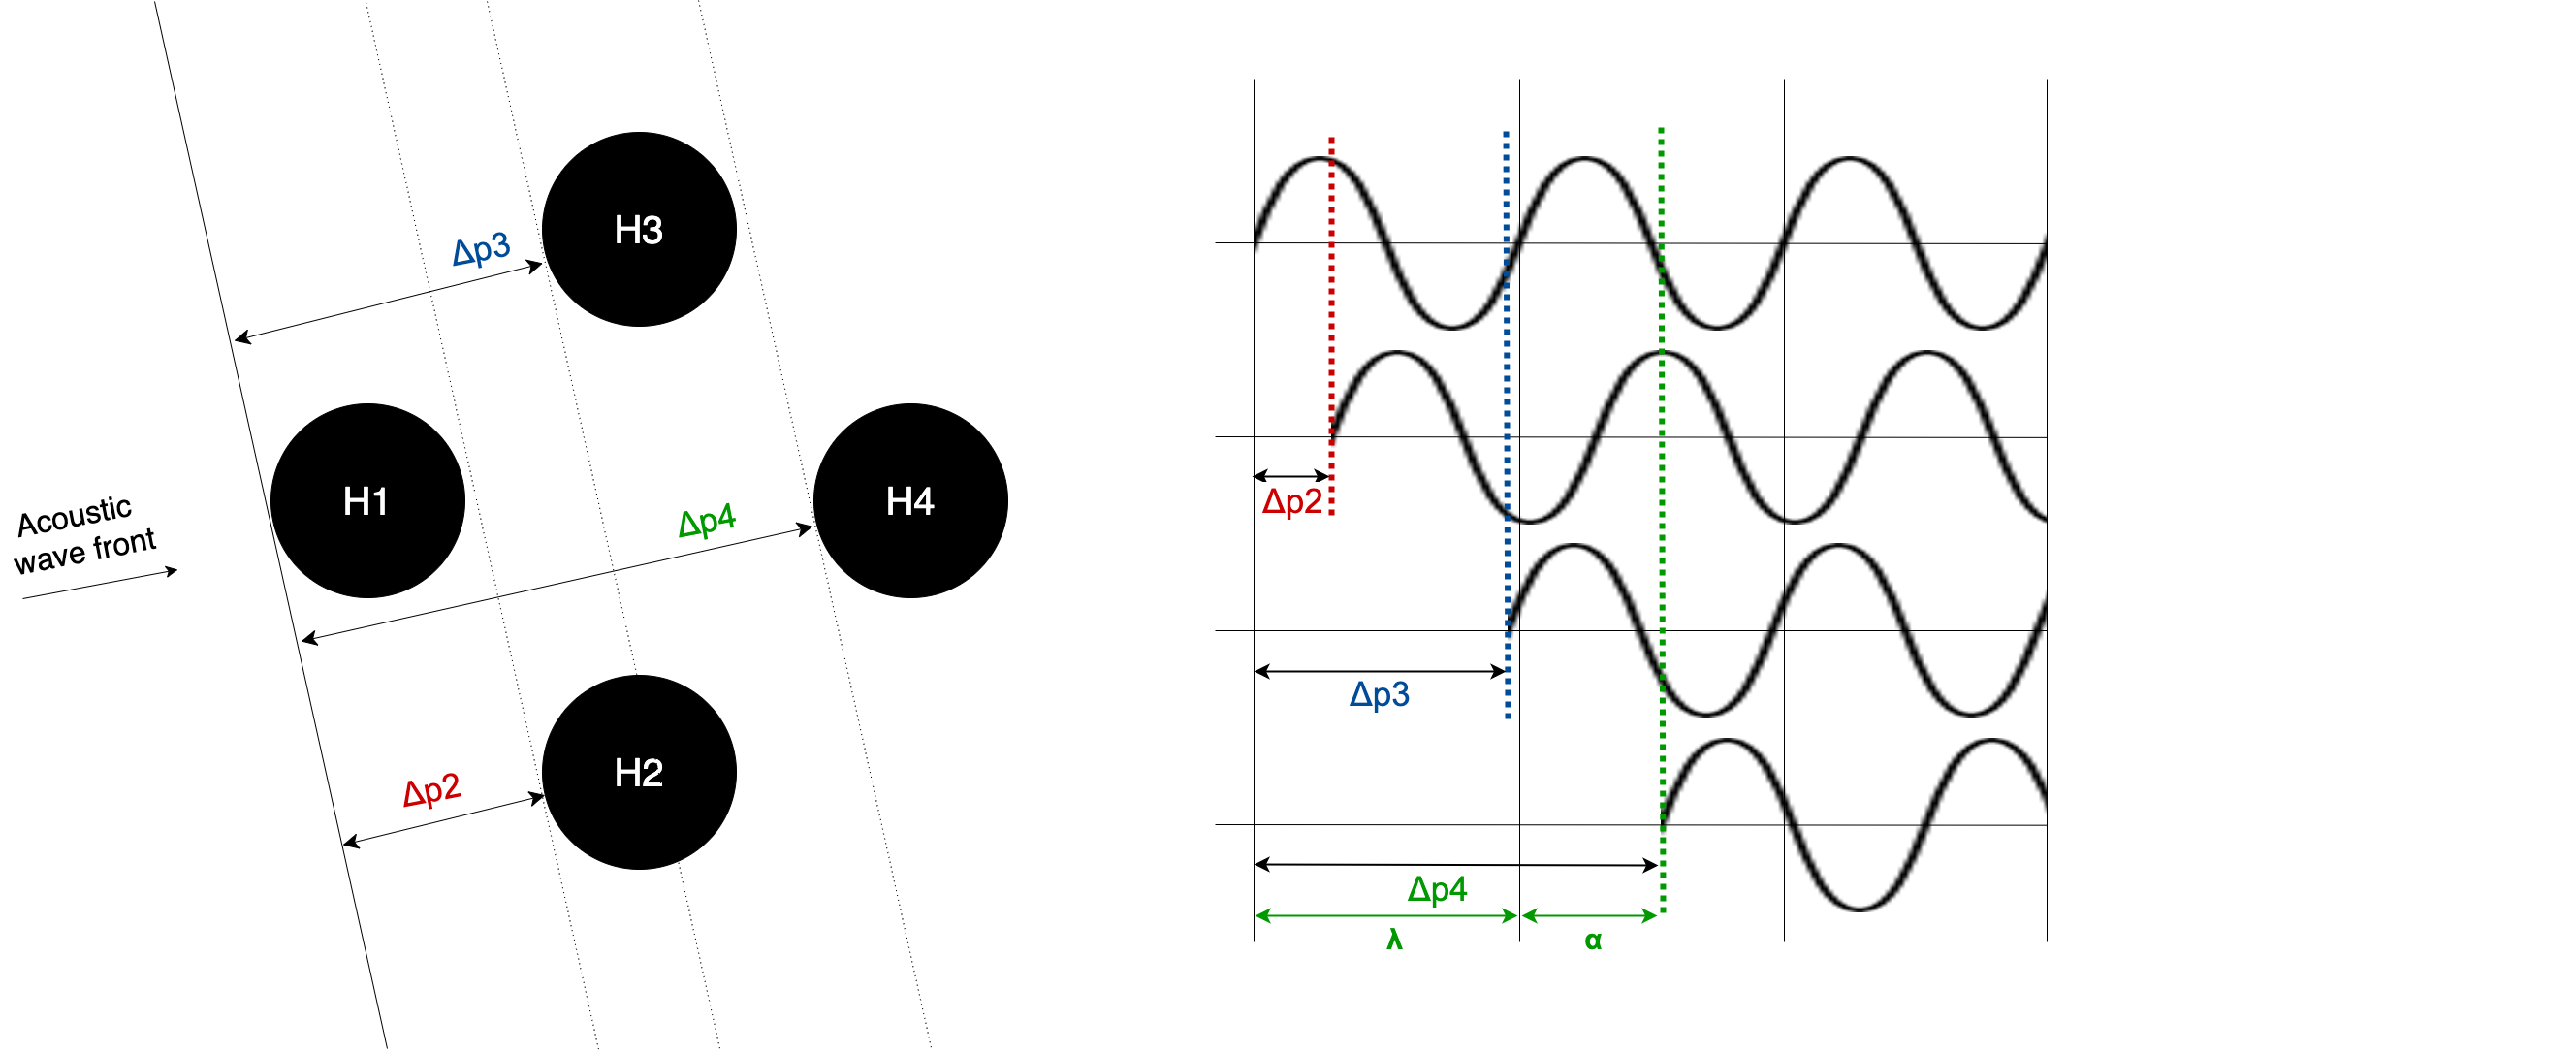
\includegraphics[width=1.2\textwidth]{figures/phase-diff}
	\caption{Phase difference to reference point and phase ambiguity}
	\label{fig:phasediff}
\end{figure}

For this reason, it is crucial to consider that the phase difference is given by the obtained phase value added by the number of periods ahead from the considered reference period.

In the system under study, the transmitted signal is a pure sine wave with a frequency of 24.4 $kHz$. The corresponding signal period is $T = \frac{1}{24400} $ seconds which, considering the typical underwater acoustic speed $c_s$ equal to 1500 $m/s$, the wavelength is approximately equal to $\lambda = \frac{T}{c_s} = 6.1 cm$. Having this into consideration, after obtaining the time of arrival to each hydrophone given by the cross correlation instances, besides the reference one, it is possible to conclude if the phase shift is superior to one period by analyzing if the time difference is greater than the duration of one period $T$. In figure \ref{fig:phasediff}, each mentioned time difference $\Delta t_2$, $\Delta t_3$ and $\Delta t_4$, between $H_1$ and $H_2$, $H_3$ and $H_4$ is converted to the corresponding phase differences.

One possibility to solve phase ambiguity in this system would be to place the four hydrophones with a baseline spacing inferior to $\frac{1}{2}$ of a wavelength, since the maximum reached by phase difference is 180 degrees. This way it would be possible to immediately deduce the phase difference since it would always be contained in one period. However, positioning the hydrophones closer together leads to smaller  values, causing an increase on the estimation error due to varying environment conditions (briefly enumerated in \ref{subsec: acoustic-channel}). Additionally, since the hydrophones to be used in this system have a corresponding diameter of roughly half of a wavelength, they would not allow to execute the mentioned configuration and so this possibility will not be contemplated.

In order to compensate this phase ambiguity, a simple relation was developed which allows to calculate the absolute time difference between the moment a signal is received by hydrophone A, $T_A$, and when the same signal is received by a further hydrophone B, $T_B$. Figure \ref{fig:ambiguity} illustrates this association, where the represented sinusoidal waves correspond to the same signal arriving at hydrophones A and B. 

\begin{figure}[!htbp]
	\centering
	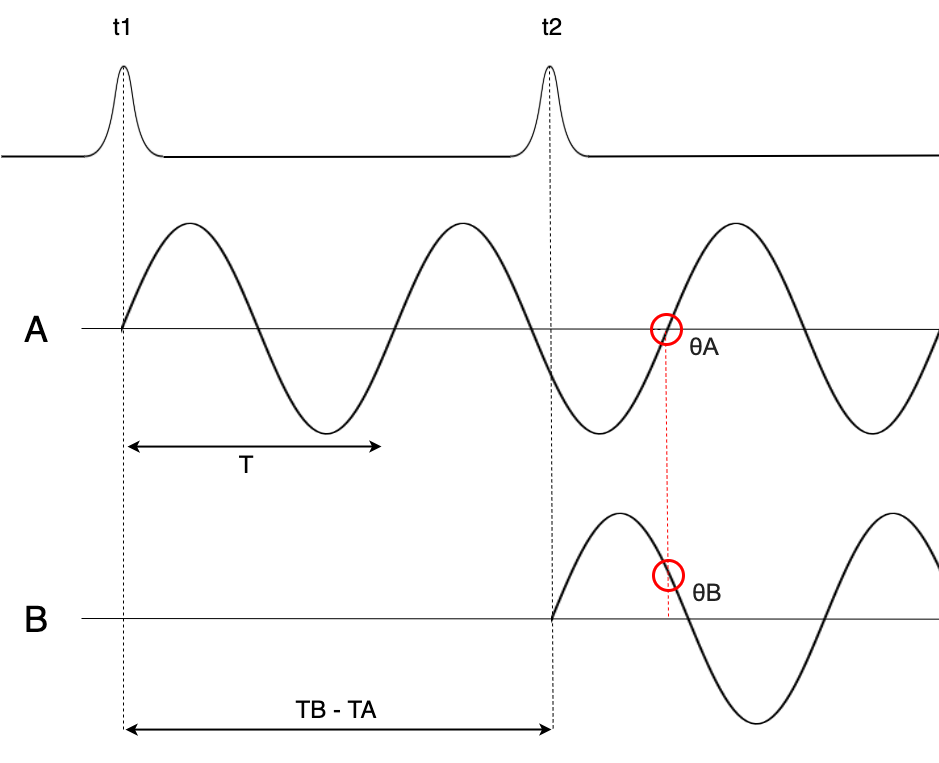
\includegraphics[width=0.6\textwidth]{figures/ambiguity}
	\captionsetup{justification=centering,margin=2cm}
	\caption{Ambiguity correction through correlation and phase difference}
	\label{fig:ambiguity}
\end{figure}

This correspondence uses the time stamps obtained by the correlation peaks combined with the calculated phase difference, that is determined in parallel, so that the measurement is more accurate. Equation (\ref{eq:phase-amb}) translates this relation, where $t_1$ and $t_2$ are the correlation peaks obtained from the signal arriving at hydrophone A and B, respectively, and so by rounding for the next integer number the difference between the correlation peaks, $t_2 - t_1$, we will obtain in which period, $T$, of signal in A will the signal in B arrive. Then the measurement is improved by subtracting a phase difference, $\theta_B - \theta_A$, so that the instant at which the signal is detected in hydrophone B can be defined. 

\begin{eqnarray}
	& T_B - T_A = round(\frac{t_2-t_1}{T}) - (\theta_B - \theta_A)
	\label{eq:phase-amb}
\end{eqnarray}

\subsection{Doppler Effect}

The implemented process uses the information of the transmitted signal's operating frequency in order to compute the phase differences and determine the overall times of arrival. However, in real scenarios the environmental conditions can distort this frequency between the source and the receiver. In the present study, since the vehicle is predominantly moving, then the Doppler effect could influence the signal's frequency, leading to erroneous calculations.

In order to evaluate if the Doppler effect influences the system, it is possible to calculate the frequency deviation observed for a known relative speed between vehicles. Considering that the relative speed between the transmitter and the receiver is denoted as $relative\_speed$ and using a fixed sound speed, $c_s$, with a determined frequency of the transmitted signal, the relation (\ref{eq:doppler}) can be established. 

\begin{eqnarray}
	&freq\_deviation = \frac{relative\_speed}{c_s} \times signal\_freq
	\label{eq:doppler}
\end{eqnarray}

Therefore, considering the frequency of the signal equal to $24.4kHz$ and a $c_s$ of $1500 m/s$, it is observable that the frequency deviation will be dependent on the relative speed. Considering a transmitter that is static and a typical value for the navigation velocity of an AUV around $2 m/s$, which results in a frequency deviation of approximately $32.5Hz$. This allows to consider the Doppler effect negligible in this case.

A way to prevent this deviation is to integrate a frequency detector which senses the relative navigation speed in real time and adapts the used frequency. This mechanism is not integrated in the present research work.